\newpage
\clearpage
\pagenumbering{arabic}

% -------------------------------------------------------------
% --------------------- LECTURE 1 23/10 -----------------------
% -------------------------------------------------------------

%TODO I would label and caption the figures so they can be referenced and they can appear wherever TeX thinks best /William

\chapter{Why should you care? An informal introduction}
%As the name suggests, this subject is two-sided: we have a physics part, namely Quantum Field Theory, and a mathematics part, more specifically topology and in particular (Co)Bordism. Let us explore the motivations and ideas behind these two subjects and how they come together. Do not worry if everything is not immediately clear, it will become so during the semester... hopefully. /// Andre: there is nothing wrong with this, just liked more the alternative I wrote down, feel free to change it back /AAndre
There are two ways one can see topological field theories:
\begin{enumerate}
    \item As a way to make (some\footnote{Sadly, TFTs cannot axiomatize many quantum field theories that are particularly useful in physics, e.g. the quantum field theory behind the standard model.}) quantum field theories more mathematically rigorous
    \item As a way to refine bordism invariants
\end{enumerate}
We now sketch how these two approaches work.
\section{QFT}
\epigraph{Physics is very interesting:
There are many, many interesting theorems.
Unfortunately, there are no
definitions.}{David Kazhdan}
\noindent Start with a (smooth) manifold $M$ and, generally, some extra structure. For example:
\begin{itemize}
    \item $M^4=\R^4$ with a metric with signature $(+, +, +, -)$, so that we can distinguish a strictly spatial part and a temporal part $(\R^4=\R^3_{space}\times\R^1_{time})$. This is called \textit{Minkowski Spacetime} and is particularly important in QFT being the geometric foundation of Special Relativity,
    \item $M^3=\R^3$ with the Euclidean metric,
    \item $M^2$ with a conformal structure,
    \item $M^{11}$ as an ``Elliptic Fibration'', something which \textit{locally} looks like $\left(S^1\times S^1\right)\times \ something$. These things are useful in areas with high-sounding names such as ``M-Theory'' or, more generically, ``String Theory''.
\end{itemize}
However, in general, these manifolds must be thought of with other structures, like connections, bundles...\\
Now we can ``define'' a Quantum Field Theory on $M$ via a list of ingredients:
\begin{enumerate}
    \item \textbf{\textit{Fields}}. The \underbar{space} of fields $\mathcal{F}$, associated usually to a bundle $E\xrightarrow{p}M$, is defined as sections\footnote{A section of a bundle $E\xrightarrow{p}M$ is a map (in this context, smooth) $s:M\to E$ such that $p\circ s=id_M$.} of $E$ over $M$. In the case the bundle is trivial ($E\cong M\times X$), then $\mathcal{F}=\Gamma(M,E)=\text{Maps}(M\rightarrow X)$. But what mathematical object are we dealing with? What do we mean by ``space'' here? Is it a set, a topological space, a category, a scheme, a stack...?\\
    \begin{figure}[!ht]
        \centering
        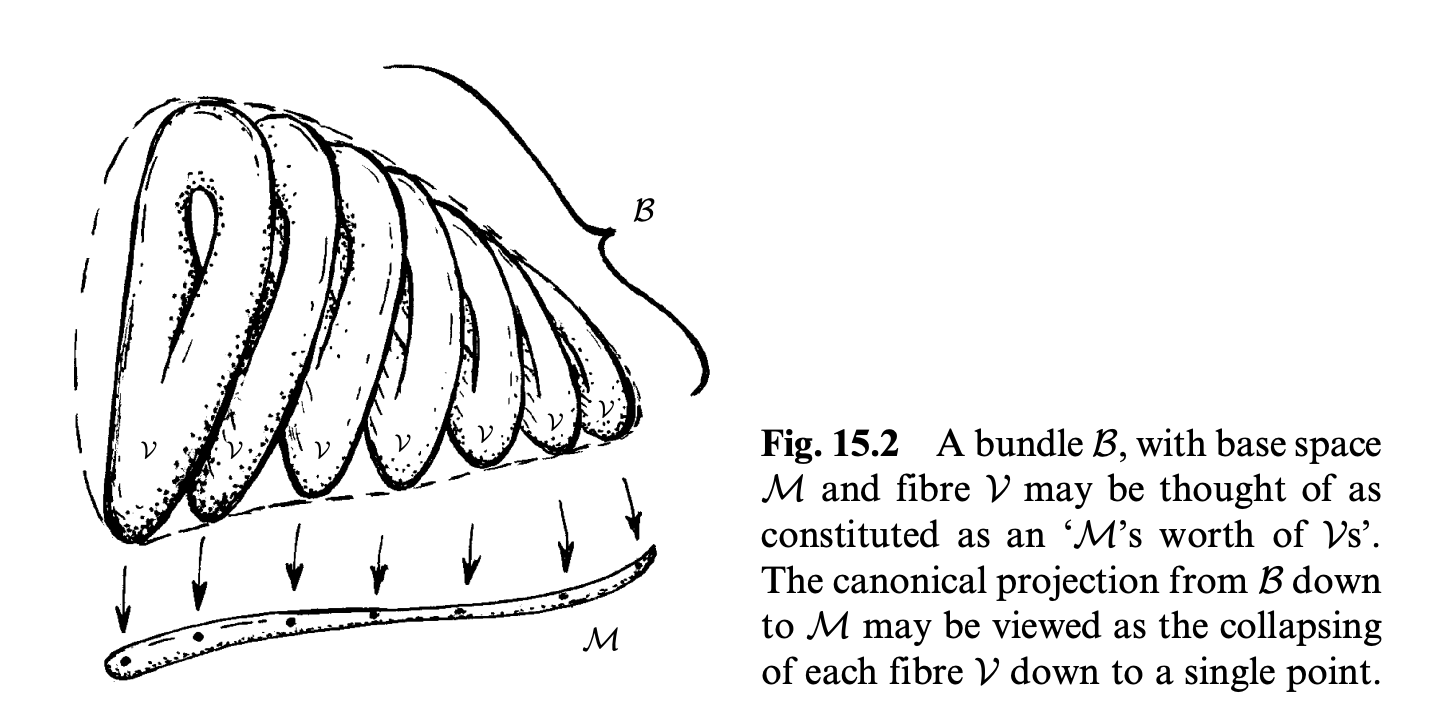
\includegraphics[width=8cm]{images/Lecture 1/penrose.png}
    \end{figure}
    %
    \item \textbf{\textit{Partition Function}}. We need a measure against which we can compute
     ``correlation functions'' of fields $\psi_1,\psi_2$ i.e. the ``likelihood of $\psi_1$ given
      $\psi_2$''. We thus define a Partition Function
    $$Z(M)=\int_{\psi\in\mathcal{F}}\ e^{iS(\psi)}\mathcal{D}\psi,$$
    with
    $$S(\psi)=\int_M \mathcal{L}(\psi),$$
    called the Action Functional. Generally $\mathcal{L}$ is a polynomial in the fields and it has derivatives. From the Partition Function one can obtain the correlation functions. Although physicists use this formula all the time, formally there is a problem: the measure $\mathcal{D}\psi$ is, in most cases, ill defined.
    \begin{figure}[!ht]
        \centering
        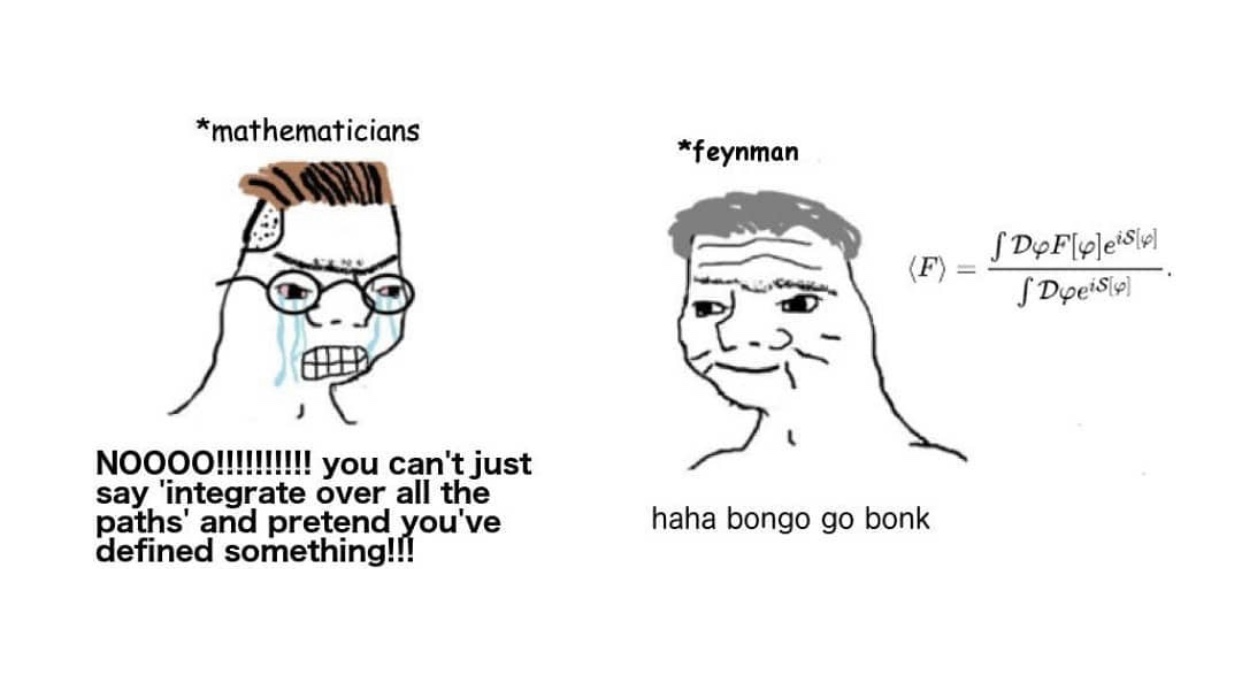
\includegraphics[width=9.2cm]{images/Lecture 1/feynman.png}
    \end{figure}
    %
    \item \textbf{\textit{Quantization}}. Often QFT arises from ``quantizing'' something classical. But what does this mean? And in what way does this thing behave when changing input?
\end{enumerate}
Physicists use all sorts of techniques (Feynman Diagrams, renormalization...) to make sense of undefined measures and divergences of all kinds emerging from calculations, dealing with things like $\infty-\infty$ or $\infty/\infty$ and obtaining finite and testable results.

\noindent This black box that physicists have (successfully) developed frustrates mathematicians because they do not understand why it works!
Therefore, axiomatizations have been developed exploiting new tools from geometry, algebra and topology to develop a formal and rigorous framework\footnote{More specifically to the path integral, see \cite[2.1]{Carqueville_2018} for an introduction on how topological field theories can be seen as a way to axiomatize some properties of the path integral as a tool to compute correlation functions.}.

\noindent The Partition Function $Z$ behaves well when ``smoothly'' changing the metric and is (in most cases) independent of most extra data of the manifold, so $Z(M)$ depends only on the smooth manifold and as such is purely topological!

\bigskip

If someone is into mathematics for the money or the prestige\footnote{If not already sufficiently clear, we explicitly state that this is a joke.}, the field of topological field theories is the one to specialize in:
 \begin{itemize}
    \item René Thom, the mathematician who laid the foundation of cobordism theory\footnote{Which is at the root of TFTs: TFTs can be seen as a refinement of his work.} in his PhD thesis, received the Fields Medal for this.
    
    \item Shiing-Shen Chern and Jim Simons discovered geometric invariants of 3-dimensional Riemannian manifolds called (classical) Chern-Simons invariants. They are a generalization of the total geodesic curvature, which is in turn a generalization of the curvature of a plane curve that $=0$ when the curve is a geodesic. Such invariants are the basic building blocks Witten used to define the earliest example we have of a TFT: 3d Chern-Simons theory\footnote{One can find more on this in \cite{freed2008remarks}}. Simons  then went on to found an incredibily successful hedge fund and became a billionaire. Chern continued to do groundbreaking work in differential geometry and topology; so much that some years ago the International Congress of Mathematicians named a prize after him: the \hyperlink{https://en.wikipedia.org/wiki/Chern_Medal}{Chern Medal}.
    \item Edward Witten received his Fields medal mainly because he found a link between 3d-TFTs, in particular Chern-Simons theory, and knot theory, in particular with the Jones polynomial. See \cite{Witten1989} for details.
\end{itemize} 
The Jones polynomial is a topological invariant of a knot, meaning that you can assign to each knot a Jones Polynomial in such a way that if two Knots have different polynomials, then they must be different.
\begin{center}
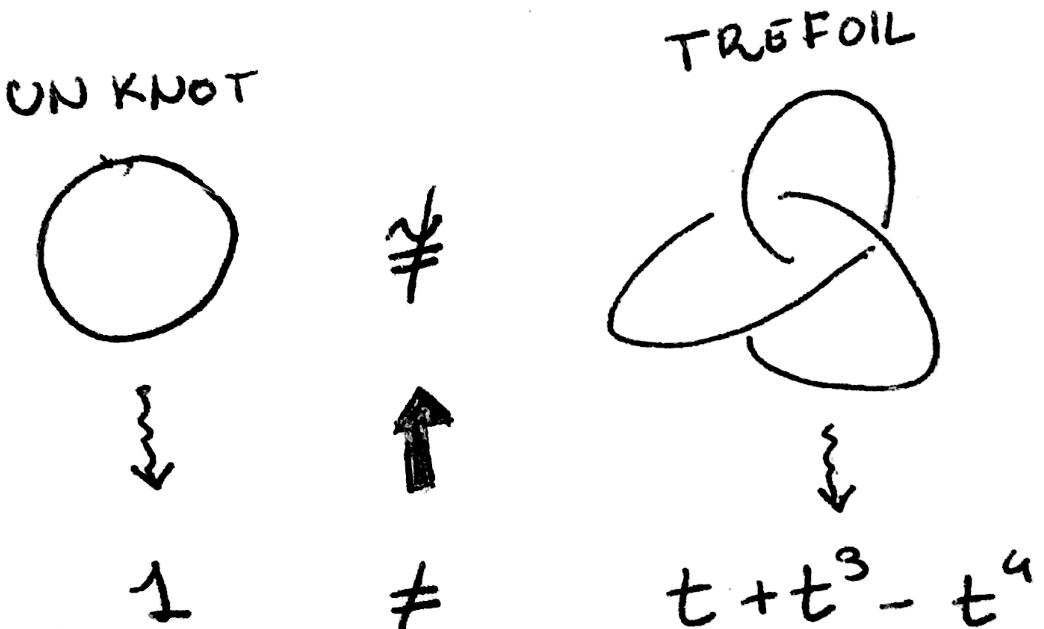
\includegraphics[width=5cm]{images/Lecture 1/Jones.jpg}
\end{center}
What the heck do TFTs and knots have in common?! There is actually a deep connection between the two.
When writing his paper, Witten drew several pictures like the following:
%The order of the images is compiled strangely
\begin{center}
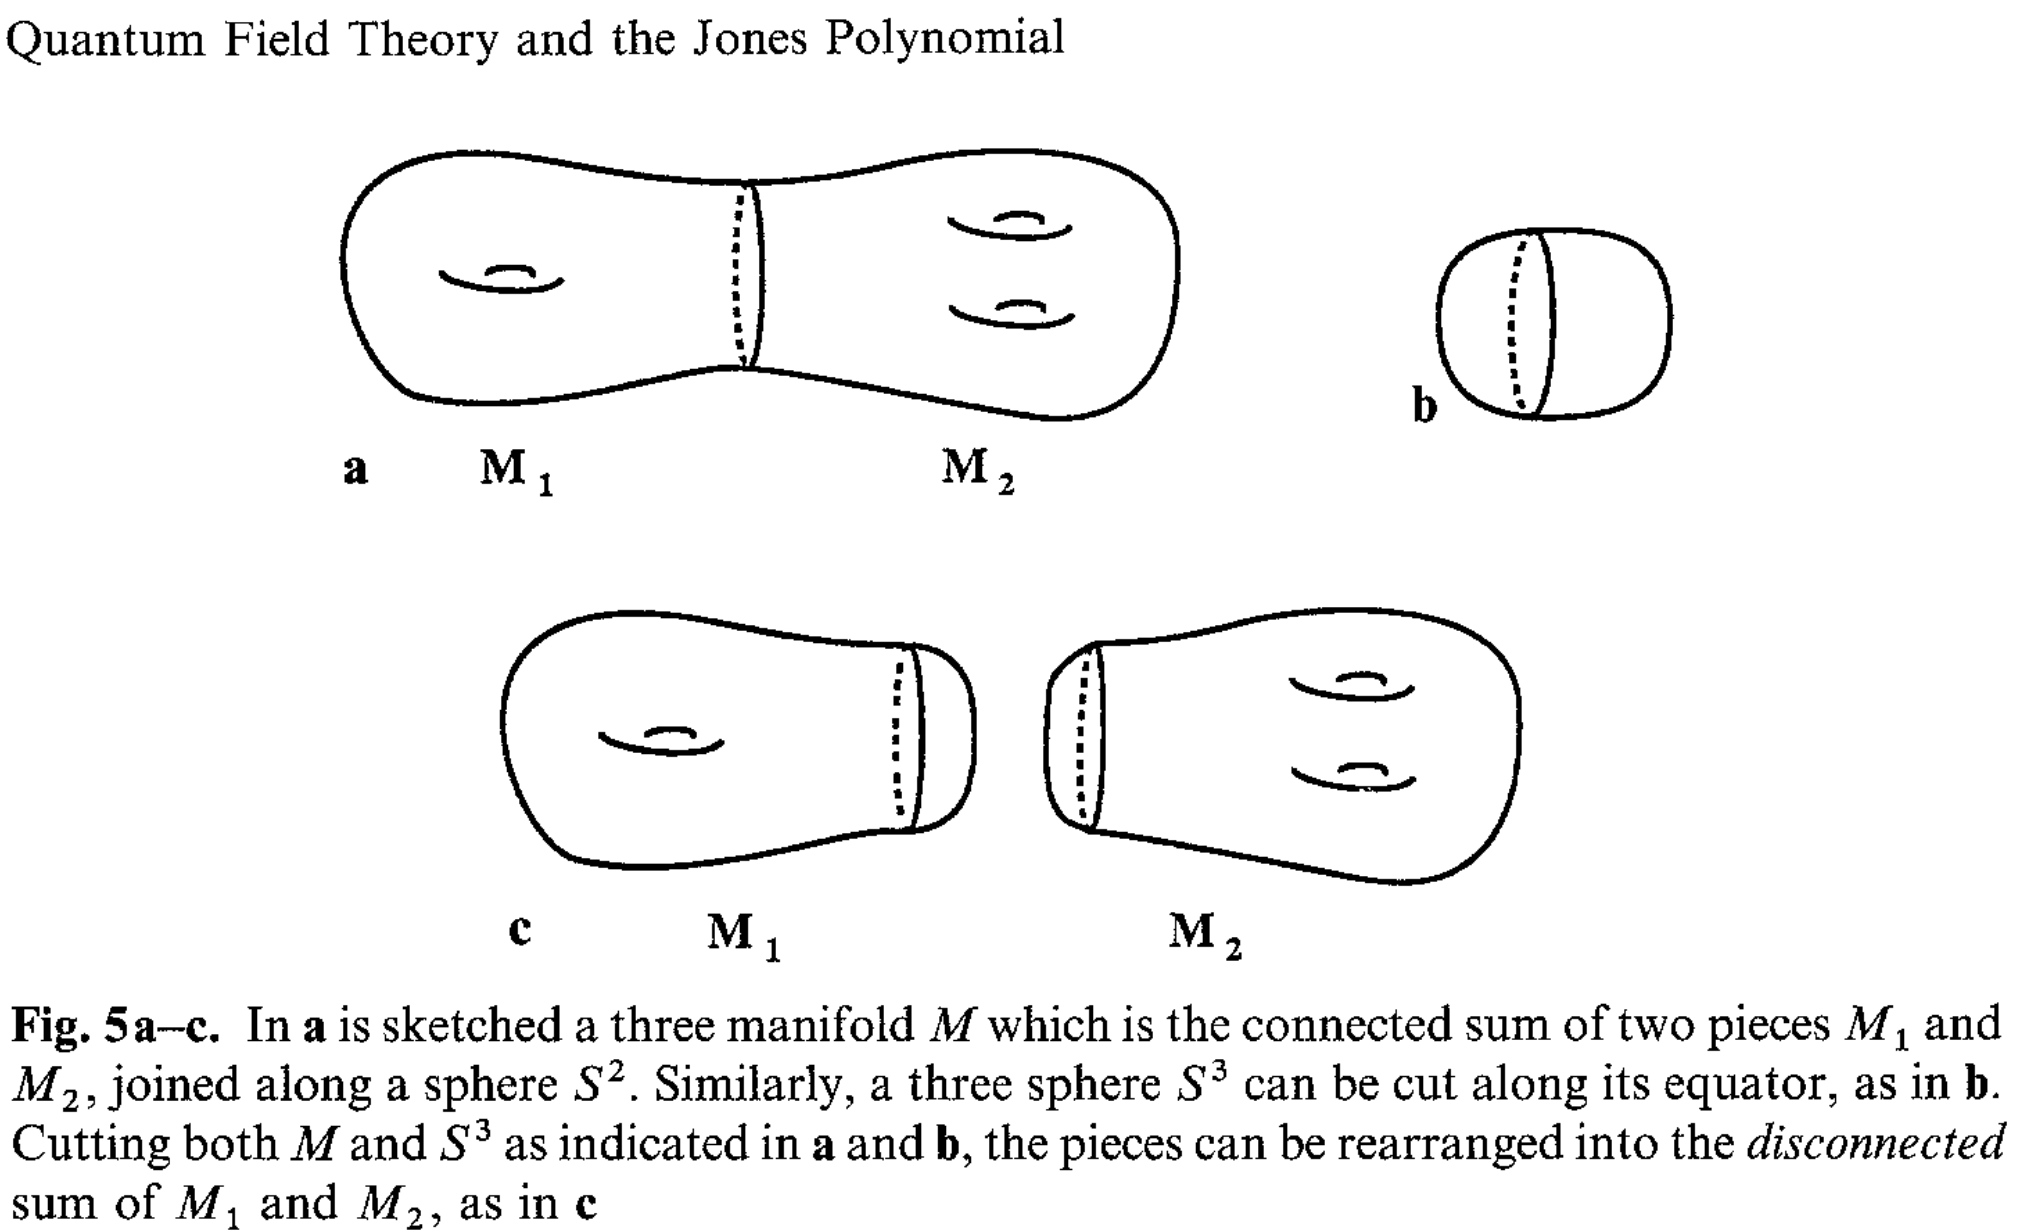
\includegraphics[width=10cm]{images/Lecture 1/witten.png}
\end{center}
Two mathematicians, Segal and Atiyah, recognized a hidden symmetric monoidal functor and pinned down  Witten's intuitions rigorously, thereby axiomatizing TQFTs (and CFTs).

\section{Topology}
\begin{flushleft}
\epigraph{Topology is the science of fundamental patterns and structural relationships of event constellations.}{Fuller}
\end{flushleft}
The ideas behind cobordisms were developed already by Poincaré together with homology (and their group structure was discovered and investigated by Emmy Noether) but a proper definition was established by Pontryangin and Thom in the 20$^{\text{th}}$ century.

The strategy in general in (algebraic) topology is to probe a topological space by mapping into it, a way of viewing things very reminiscent of the Yoneda Lemma.
In the case of (singular) homology, we map simplices into the space of interest $S$. These maps are indexed by the dimension of the simplex as in the following figure.
\begin{figure}[!ht]
\centering
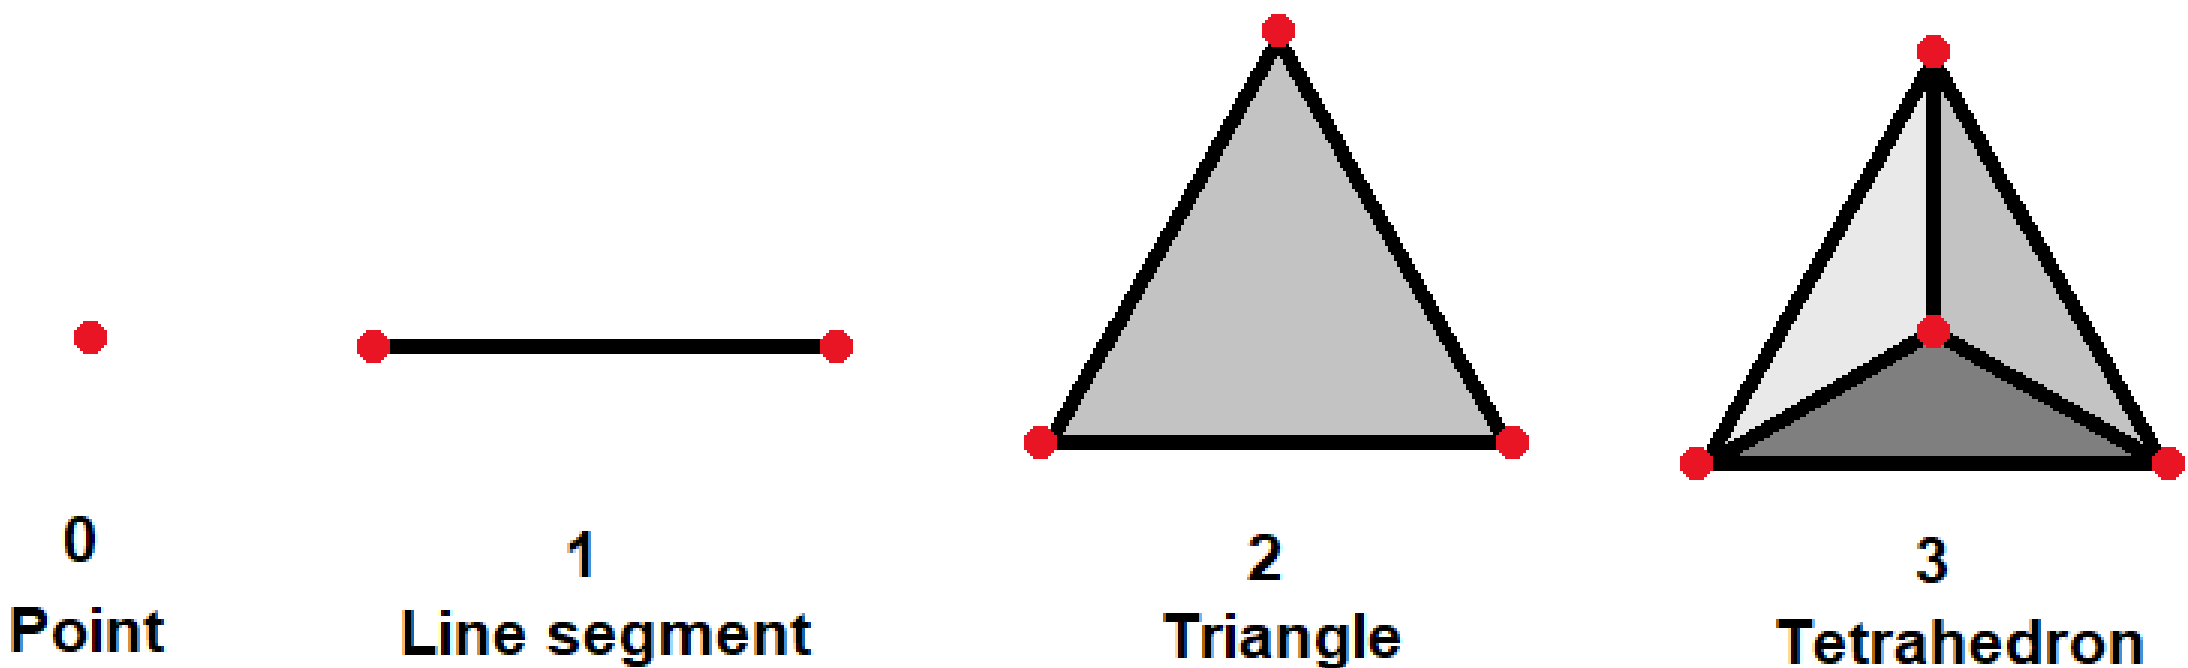
\includegraphics[width=6.5cm]{images/Lecture 1/simplex.png}
\end{figure}
We want to construct an algebraic structure around these maps $\sigma^{(n)}:\Delta^n\to S$ and so we  choose a set of coefficients, say $\R$, and construct the set of ``formal (finite) sums''  of $n$-simplices as
$$\sum a_i\sigma^{(n)}_i  ,$$
with $a_i\in\R$ and call this set $C_n(S)$. This is now an $\R$-Vector Space generated by the simplices. On the set of simplices we can introduce a map $\partial$, often called the differential or boundary, that takes each simplex to the alternating sum of the $n-1$ simplices that make up its boundary:
$$\partial\sigma^{(n)}:=\sum_{i=0}^{n}(-1)^i\sigma^{(n)}|_{i^{\text{th}}-boundary} \ ,$$
and then extend it linearly to $C_n(S)$. Calling $\partial_n:=\partial|_{C_n(S)}$, we have $\partial_n:C_n(S)\to C_{n-1}(S)$ and it can also be shown that $\partial_n \circ\partial_{n+1}=0$, a property which is often simply written as $\partial^2=0$. This defines a chain complex structure.
Given this property of $\de$, note that $\text{im}(\partial_{n+1})\subset \text{ker}(\partial_n)$ and therefore, we can define the $n^{\text{th}}$ homology of $S$ as
\begin{equation*}
    H_n(S)=\Big\{c^{(n)}: \ \ \partial_n c^{(n)}=0\Big\}\big{/}\Big\{f^{(n)}: \ \ f^{(n)}=\partial_{n+1} (f'^{(n+1)})\Big\}=\frac{\text{ker}(\partial_n)}{\text{im}(\partial_{n+1})},
\end{equation*}
and this is a vector space (by construction).
\begin{figure}[!ht]
\centering
\captionsetup{labelformat=empty, format = hang}
\begin{measuredfigure}
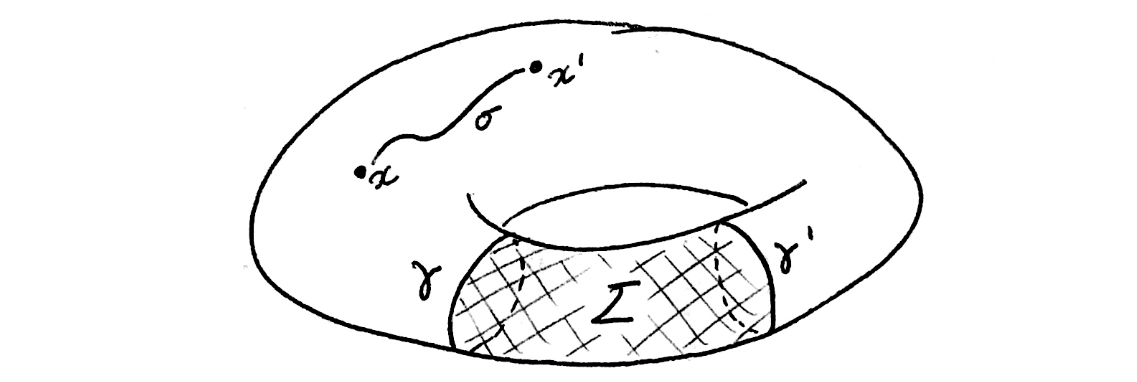
\includegraphics[width=10.40cm]{images/Lecture 1/homology.jpeg}
\caption{\small{Note that $x-x'=\partial\sigma$ so $x$ and $x'$ define the same element in $H_0$, similarly $\gamma-\gamma'=\partial\Sigma$ so that $\gamma$ and $\gamma'$ define the same element in $H_1$.}}
\end{measuredfigure}
\end{figure}

The elements of $H_1(S)$ and $H_2(S)$ can be characterized in different ways:
\begin{enumerate}
    \item The elements of $H_1(S)$ can be represented by a collection of oriented loops mapped in $S$.
    $$\amalg \ S^1\longrightarrow S$$
    \item The elements of $H_2(S)$ can be represented by a collection of maps from closed oriented surfaces (e.g. genus $g-$surfaces) in $S$.
    $$\amalg \ \Sigma\longrightarrow S$$
    \item Let $c\in H_1(S)$, then $\partial c=0$. Now by $1.$ this is some map $c: \amalg \ S^1\to S$ which is $0 \in H_1(S)$ if and only if it extends to a map $\tilde c$ of oriented surfaces in $S$, i.e. if there is the map on the bottom right such that the following diagram commutes.
    $$
    \begin{tikzcd}[row sep=tiny, column sep=small]
      \amalg \ S^1 \ar[drrr, "c"] \ar[dd, hook]\\
                  &&&S \\
      \amalg \ \Sigma \ar[urrr, dashrightarrow, "\tilde c"']
    \end{tikzcd}
    $$
    
    A drawing might be helpful:
    \begin{figure}[!ht]
    \centering
    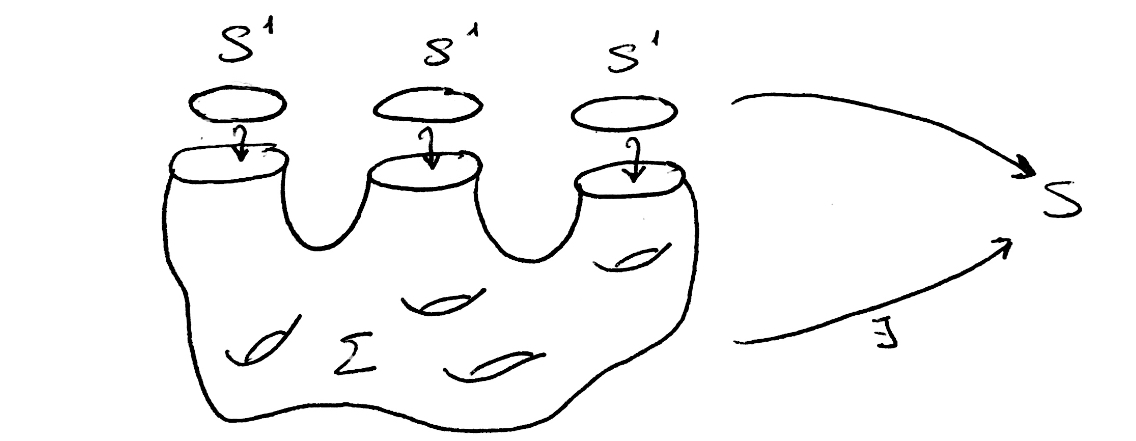
\includegraphics[width=11cm]{images/Lecture 1/extension.png}
    \end{figure}
\end{enumerate}
Can we then construct something like homology but characterized more like this last property?
This is exactly the idea of \textit{(co)bordism}:
\begin{enumerate}
    \item Let $M^n$ be a $n-$dimensional smooth compact manifold generally with boundary. Now, instead of maps from simplices we consider maps
    $$M^n\xrightarrow{f} S.$$
    \item Instead of the boundary map of simplices we consider something like:
    $$\partial\big(M^n\xrightarrow{f}S\big)=\big(\partial M^n\xrightarrow{f|_{\partial M^n}}S\big),$$
    where, if $\partial M^n=\emptyset$ then define the map to be $0$.
    \item Let $H^{\text{bord}}_n(S)$ denote this ``homology theory'' of degree $n$ on the space $S$. Let $M^n$ be closed, then $M^n\xrightarrow{f} S$ is zero in $H^{\text{bord}}_n(S)$ if and only if the map $f$ extends to a $(n+1)-$dimensional smooth compact manifold $W$ such that $\partial W= M$.
\end{enumerate}
Using these ideas one obtains something very similar to singular homology even though different, indeed this bordism theory constitutes a generalized homology theory\footnote{There exist a list of axioms called \textit{Eilenberg–Steenrod axioms} that is used to define what a homology theory is since it may come in different flavours. A generalized homology theory is a theory that has every property required but one, generally (as in the case of Bordism as seen below) that one is the \textit{dimension axiom}.}! 

\medskip

In particular, consider the one point space $S=\{*\}=pt$. What are elements in $H^{\text{bord}}_n(pt)$?

\noindent Consider a closed manifold $M^n$. This defines a class in $H^{\text{bord}}_n(pt)$ since $\de M^n = \emptyset$. Now, this is $0 \in H^{\text{bord}}_n(pt)$ if we can find a compact $n+1$ manifold $W^{n+1}$ and maps into $pt$ such that the following diagram commutes
\begin{equation*}
    \begin{tikzcd}
        M^n \arrow[dd,  hook] \arrow[rd, dashed]                         \\
                                                & pt \\
        W^{n+1} \arrow[ru, dashed] 
    \end{tikzcd}
\end{equation*}
however the maps into $pt$ are trivial and carry no extra information. 
Now, ``surely'' not all closed manifolds are a boundary of compact manifold! And so we can be sure that, in general, $H^{\text{bord}}_n(pt)\neq0$ for $n>0$.

\medskip

But when do two $n$-manifolds represent the same class in $H^{\text{bord}}_n(S)$? In the case of $S = pt$, they should be the boundary of the same manifold. In general, we require also that the maps into $S$ extend to the $n+1$ manifold, i.e. let $M_1$ and $M_2$ be closed $n$ manifolds, with maps $M_1\xrightarrow{f_1}S$ and $M_2\xrightarrow{f_2}S$, then they represent the same element in $H^{\text{bord}}_n(S)$ if and only if there exists a compact $n+1$ manifold with boundary $W$ with a map $ W\xrightarrow{g}S$ with the property that $\partial W= M_1 \amalg M_2$ and such that it makes the following diagram commute
    $$
    \begin{tikzcd}
M_1 \arrow[rd, hook] \arrow[rrd, bend left, "f_1"' description]         \\
                                        & W \arrow[r, "g"] & S \\
M_2 \arrow[ru, hook] \arrow[rru, bend right, "f_2" description]         
\end{tikzcd}
    $$
Pictorially
\begin{figure}[!ht]
\centering
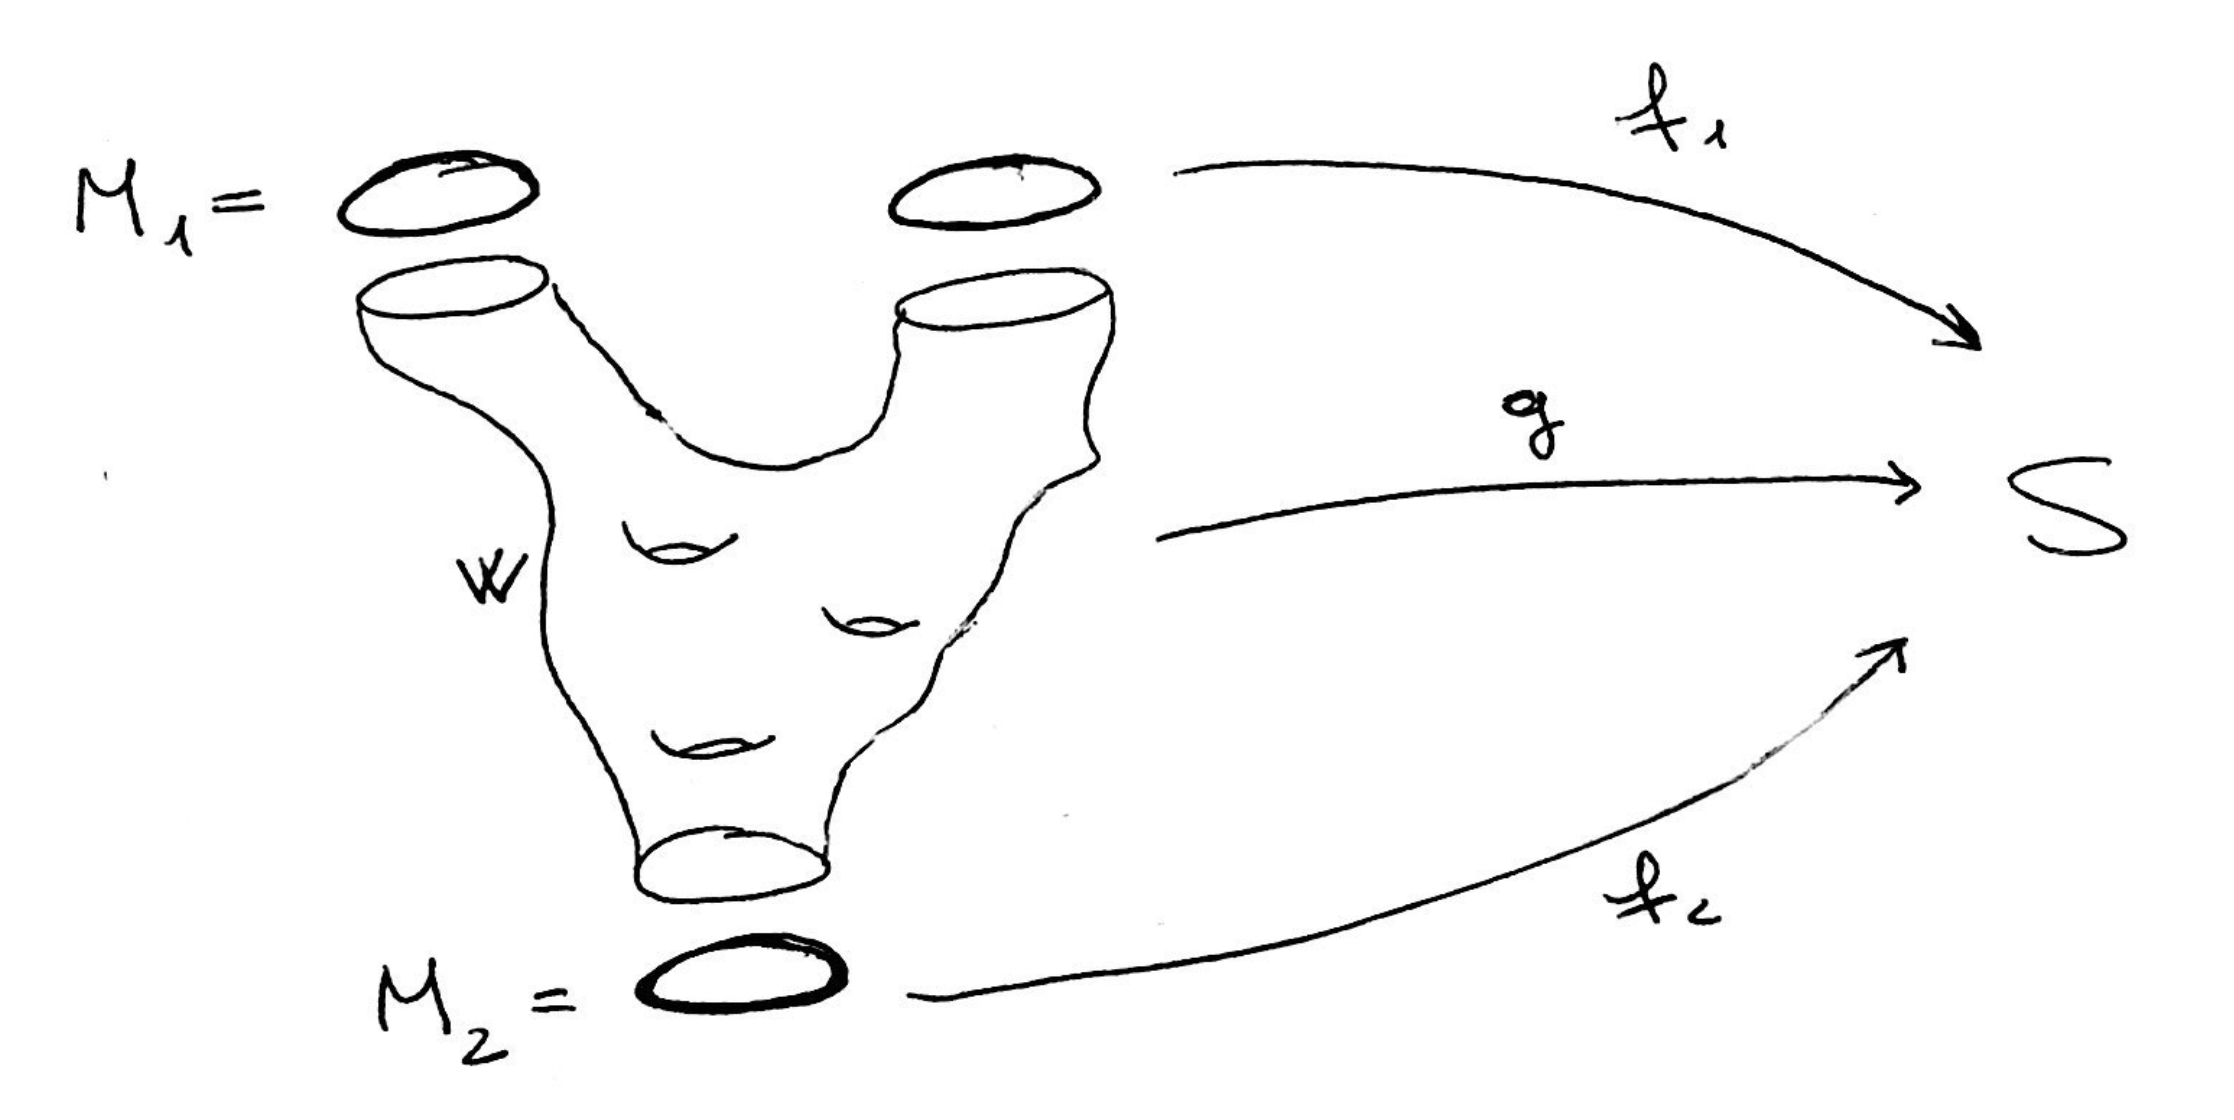
\includegraphics[width=10cm]{images/Lecture 1/cobordism.png}
\end{figure}
We then say that $M_1$ and $M_2$ are \textit{cobordant} and $W$ is called a \textit{bordism} from $M_1$ to $M_2$. 

Restricting to $S= pt$ allows us to define the \textit{Cobordism Group}
$$\Omega_n=
H^{\text{bord}}_n(pt)=
\bigg\{\text{Closed $n$ manifold}\bigg\}
\bigg{/}
\biggl\{(n+1)\text{ dimensional bordisms}
%\begin{array}{l}
%\text{Cobordant Compact}\\
%\text{$(n+1)$ manifolds}
%\end{array}
\biggl\}.$$
But are all these notions are actually useful? Well, classifying manifolds up to diffeomorphism is hard: dimension $0, 1$ and $2$ can be done without too much trouble but already in dimension $3$ things get complicated (think of the Poincaré Conjecture!)... so this classifications can be done (more easily) up to bordism!

% TBD: Could be cool to restructure a bit this subsection more geared towards TFTs rather than Bordism invariants in general because  /Andrea 